% chapter3_voorbeelden.tex
% Derde hoofdstuk - Uitgewerkte voorbeelden
% Demonstreert alle box types en grafieken

\chapter{Uitgewerkte Voorbeelden}
\label{ch:voorbeelden}

Dit hoofdstuk toont alle beschikbare omgevingen en hun gebruik.

\section{Box Omgevingen}

\subsection{Concept Box}
\begin{conceptbox}[title=Belangrijke Definitie]
Een \concept{conceptbox} wordt gebruikt voor belangrijke definities en kernbegrippen.
De blauwe accent aan de linkerkant trekt de aandacht.
\end{conceptbox}

\subsection{Theorie Box}
\begin{theorieblok}[title=Theoretisch Kader]
De \concept{theorieblok} is ideaal voor theoretische uitleg en achtergrond.
Paarse kleur onderscheidt het van definities.
\end{theorieblok}

\subsection{Oefening Box}
\begin{oefenblok}[title=Oefening 3.1]
\textbf{Gegeven:} Een massa $m = \SI{2}{kg}$ valt van hoogte $h = \SI{10}{m}$.

\textbf{Gevraagd:} Bereken de snelheid bij de grond.

\textbf{Oplossing:}
Uit energiebehoud: $E_p = E_k$
\[ mgh = \frac{1}{2}mv^2 \]
\[ v = \sqrt{2gh} = \sqrt{2 \times \SI{9.81}{m/s^2} \times \SI{10}{m}} = \SI{14.0}{m/s} \]
\end{oefenblok}

\subsection{Voorbeeld Box}
\begin{voorbeeld}[title=Praktisch Voorbeeld]
Dit is een \concept{voorbeeld} box, bedoeld voor uitgewerkte praktijkvoorbeelden.
De oranje kleur geeft aan dat het om een concreet voorbeeld gaat.
\end{voorbeeld}

\subsection{Warning Box}
\begin{warningbox}[title=Let op!]
\belangrijk{Waarschuwing}: Vergeet niet tweemaal te compileren voor het formularium!
\end{warningbox}

\subsection{Exam Box}
\begin{examenbox}
Dit is een compacte examentip. Ideaal voor korte, praktische tips.
\end{examenbox}

\section{Grafieken met TikZ/PGFPlots}

\begin{figure}[H]
    \centering
    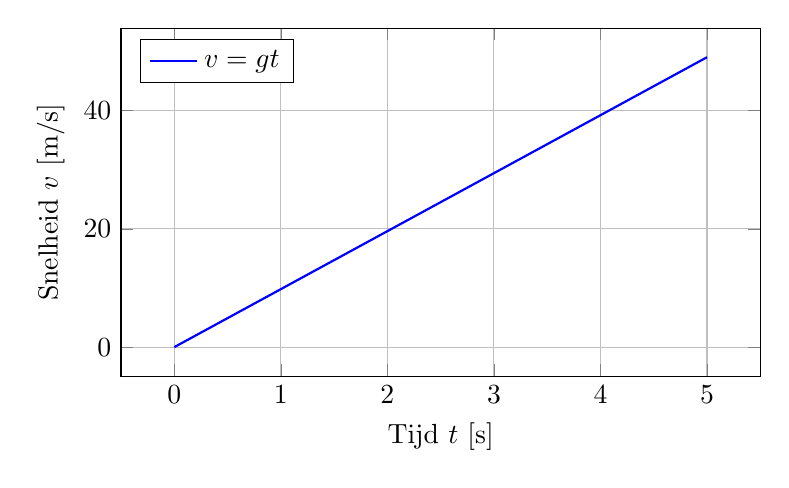
\begin{tikzpicture}
        \begin{axis}[
            width=0.8\linewidth,
            height=6cm,
            xlabel={Tijd $t$ [\si{s}]},
            ylabel={Snelheid $v$ [\si{m/s}]},
            grid=major,
            legend pos=north west
        ]
            \addplot[blue, thick, domain=0:5, samples=50] {9.81*x};
            \addlegendentry{$v = gt$}
        \end{axis}
    \end{tikzpicture}
    \caption{Snelheid bij vrije val (zonder luchtweerstand)}
    \label{fig:vrije-val}
\end{figure}

Zie \cref{fig:vrije-val} voor de grafiek van snelheid bij vrije val.

\section{Tabellen}

\begin{table}[H]
    \centering
    \caption{Fysische constanten}
    \label{tab:constanten}
    \begin{tabular}{lll}
        \toprule
        \textbf{Constante} & \textbf{Symbool} & \textbf{Waarde} \\
        \midrule
        Zwaartekracht & $g$ & \SI{9.81}{m/s^2} \\
        Lichtsnelheid & $c$ & \SI{3e8}{m/s} \\
        Boltzmann & $k_B$ & \SI{1.38e-23}{J/K} \\
        \bottomrule
    \end{tabular}
\end{table}

De waarden in \cref{tab:constanten} zijn standaard SI-waarden.
